\cleardoublepage

\chapter{Entorno de mercado}
\label{makereference4}

Para que el sistema de optimización de baterías funcione de manera efectiva, no es suficiente con disponer de la información proveniente de la infraestructura con sus sensores y señales. Como el sistema opera directamente en el mercado eléctrico, su lógica de decisión debe ser retroalimentada por un entendimiento del entorno de mercado. Por ello, los datos de mercado son una fuente de información igualmente indispensable, ya que dictan el contexto económico y regulatorio en el que se toman todas las decisiones de arbitraje, formando parte del flujo de la figura.

\begin{figure}
  \centering
  % 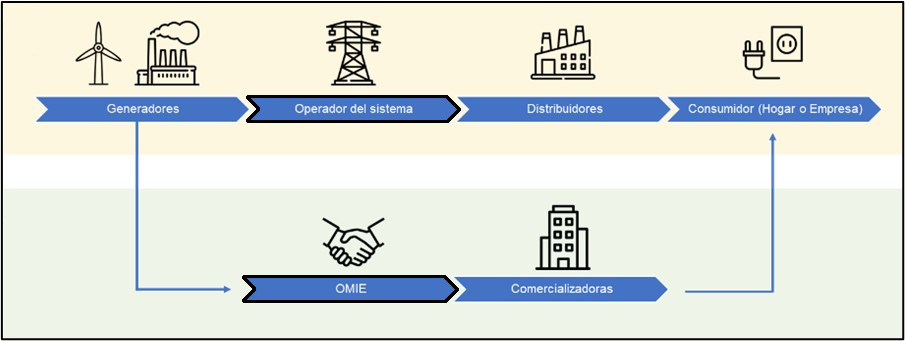
\includegraphics[width=0.5\linewidth]{figures/esquema-mercado.jpg}
  \caption{Esquema del funcionamiento del entorno del mercado.}
  \label{fig:esquema-mercado}
\end{figure}

Por tanto, se define el análisis de las fuentes de información de mercado y los procesos desarrollados para su adquisición, tratamiento e integración. Concretamente, el sistema de optimización requiere de tres categorías fundamentales de datos externos, los precios del mercado que son esenciales para formular previsiones estratégicas, la energía negociada que es clave para la liquidación de beneficios y la gestión de desvíos, y las limitaciones operativas que imponen restricciones de obligado cumplimiento.

De esta forma, se pretende describir el origen de estas fuentes de datos, las reglas que gobiernan su publicación y accesibilidad, y la arquitectura de software implementada para consumirlos de manera programática y robusta.

Para ello, primeramente se presenta al Operador del Mercado Ibérico de Energía como la fuente primordial de datos de mercado, detallando los mecanismos de obtención de precios y la naturaleza de la información de energía negociada, como se describe en el apartado~\ref{makereference4.1}. A continuación, se habla de la información proveniente de Red Eléctrica Española, que impone las limitaciones de programa de operación en tiempo real, como se explicará en la sección~\ref{makereference4.2}. Finalmente, el apartado~\ref{makereference4.3} detalla cómo se consolidan estas diversas fuentes de datos para formar una visión unificada que sirva de entrada al sistema.

Con esto, para facilitar la comprensión de las secciones posteriores, hay que dejar claro los siguientes conceptos. Las llamadas unidades físicas o UFIs representan las interfaces de intercambio de energía abstractas por encima de los flujos energéticos físicos, en donde las operaciones relizadas de una unidad física siempre deben poder respaldarse por un correcto flujo energético físicamente. Las unidades de programación o UPs son los identificadores del operador del sistema de las instalaciones al completo, y son los activos que se arbitran en el mercado, es decir, las operaciones de las unidades físicas que engloba una unidad de programación se agregan a la hora de realizar la oferta. Las unidades de oferta o UOFs son los identificadores equivalentes a las unidades de programación del operador del mercado.

\section{Operador del mercado}
\label{makereference4.1}

El Operador del Mercado Ibérico de Energía, conocido como OMIE, es la institución responsable de la gestión de los mercados spot, diario e intradiarios, de electricidad en la península ibérica. Actúa como la plataforma centralizada donde los agentes de mercado presentan sus ofertas de compra y venta de energía, y cuyo proceso de casación determina los precios y las cantidades de energía transaccionadas para cada periodo de negociación.

\begin{figure}
  \centering
  % \includegraphics[width=0.5\linewidth]{figures/omie.jpg}
  \caption{Operador del Mercado Ibérico de Energía.}
  \label{fig:omie}
\end{figure}

Por su rol como gestor y árbitro del mercado, OMIE es la fuente oficial de toda la información relativa a los resultados económicos de la operación. Cualquier sistema que pretenda participar activamente en el arbitraje energético, como el desarrollado en este proyecto, tiene la necesidad de integrarse de forma fiable y programática con los flujos de información que esta entidad publica.

Precisamente, OMIE pone a disposición la información en forma de ficheros publicados según un horario acordado tras el cierre de cada mercado correspondiente.

De esta forma, la información que el sistema desarrollado toma a través de OMIE se clasifica en dos categorías mayoritarias, los precios marginales de casación y la energía finalmente negociada por cada unidad de programación.

\subsection{Precio marginal}
\label{makereference4.1.1}

Una de las piezas de información más críticas para el sistema de optimización es la previsión de los precios a los que se liquidará la energía en los mercados futuros. Para poder realizar un arbitraje energético efectivo, posicionando estratégicamente las ofertas de compra en periodos de bajo coste y las de venta en periodos de alto beneficio, el modelo debe operar sobre una estimación fiable de dichos precios.

\begin{figure}
  \centering
  % \includegraphics[width=0.5\linewidth]{figures/precio-casación.png}
  \caption{Precio marginal de casación en el mercado.}
  \label{fig:precio-casación}
\end{figure}

Precisamente, sin esta previsión, la operación de la batería sería puramente ciega sin ningún tipo de garantías de corrección o guiado.

Por ello, para obtener esta previsión, el sistema desarrollado adopta un enfoque triple que se aprovecha de las características temporales de cada mercado.

\begin{itemize}

  \item En el mercado diario, como su variabilidad de precios entre días es significativamente mayor al resto de mercados y depende de factores del entorno más complejos (como si es fin de semana), el sistema está preparado para consumir previsiones de dos orígenes distintos. Por un lado, se puede utilizar un modelo de previsión manual en el que los agentes de mercado introducen sus propias estimaciones basadas en su experiencia. Por otro, se puede integrar la salida de un modelo de aprendizaje automático, concretamente un modelo de regresión de \textit{stacking} basado en series temporales, que ofrece una predicción automatizada.

  \item En los mercados intradiarios europeos, se ha observado empíricamente una alta correlación y una periodicidad estable entre sesiones consecutivas correspondida por lo agentes de mercado, por lo que se utiliza una previsión simple y efectiva donde el precio de casación de una sesión de mercado se emplea como la previsión para la sesión inmediatamente posterior. Así, por ejemplo, los precios resultantes del mercado intradiario 2 sirven como la entrada de previsión para optimizar las ofertas en el mercado intradiario 3.

  \item En las diferentes sesiones del mercado intradiario continuo se toma el precio de casación del último mercado disponible, sea el diario o los intradiarios. Cabe destacar que debido a la comparativamente baja liquidez del mercado continuo, la metodología de previsiones de precio descrita es la menos fiable para el mismo, aunque este aspecto negativo es contrarrestado por la suma de liquidez total de las sesiones en conjunto del mercado continuo. La razón de este comportamiento es la diferente modalidad de oferta del mercado continuo donde se ataca directamente a una oferta, por lo que no existen precios de casación globales para todas ellas.

\end{itemize}

Esta necesidad de previsión se deriva directamente del funcionamiento marginalista del mercado eléctrico. En este modelo, el precio final, conocido como precio marginal, se fija en el punto de intersección de las curvas agregadas de oferta y demanda. Dado que únicamente las ofertas de las instalaciones controladas por el sistema no tiene ni la más mínima capacidad para influir en este precio, su única estrategia viable es anticiparlo.

Afortunadamente, esta información de precios de casación es de carácter público. OMIE la publica en ficheros con una nomenclatura estandarizada, siendo el fichero marginal Programa Diario Básico de Casación (MARGINALPDBC) para el mercado diario y los ficheros marginales Programa Intradiario Básico de Casación Intradiario (MARGINALPIBCI) para los mercados intradiarios.

\subsection{Energía negociada}
\label{makereference4.1.2}

Más allá de las previsiones de precios, el sistema necesita conocer con absoluta certeza el resultado de las ofertas que ha presentado en el mercado. Existe una diferencia fundamental entre la posición óptima calculada por el algoritmo de optimización y la posición casada, que es la cantidad de energía que la instalación se ha comprometido firmemente a comprar o vender.

Esto se debe a que el funcionamiento del mercado eléctrico permite negocia la energía de un mismo periodo en múltiples ocasiones, por lo que hay que llevar la cuenta de la cantidad de la misma anteriormente ofertada.

Por ello, obtener esta información de energía negociada es importante porque permite realizar la liquidación económica real de la operación, calculando el beneficio o coste exacto a partir del precio marginal y la energía efectivamente transaccionada.

Además, es un requisito indispensable para la gestión de los desvíos y la reoptimización en mercados subsiguientes. Al conocer la energía ya comprometida, el modelo puede ajustar su plan para las siguientes sesiones, minimizando así las más costosas penalizaciones por desvío que se producen al no cumplir con el programa de energía comprometido.

Precisamente, esta discrepancia entre lo ofertado y lo casado puede deberse a múltiples factores, como que el precio de oferta no resulte competitivo y la oferta sea rechazada en su totalidad, o que se produzca una casación parcial en la que solo una fracción de la energía ofertada es aceptada por el mercado. Esta es la razón de la necesidad de tener que consultar con OMIE y no poder fiarse de la posición optima obtenida del sistema.

Pero, a diferencia de los precios, la información de energía casada es de naturaleza confidencial. Para proteger las estrategias comerciales de los participantes, OMIE la publica desglosada por unidad de programación, y cada agente de mercado solo tiene acceso a la información de sus propias unidades. Los ficheros que contienen esta información son el Programa Diario Básico Final (PDBF) para el mercado diario y el Programa Intradiario Base de Casación Acumulado (PIBCA) para los mercados intradiarios.

\section{Operador del sistema}
\label{makereference4.2}

Mientras que OMIE gestiona el componente económico del mercado, la responsabilidad de garantizar la seguridad y la estabilidad física del sistema eléctrico en tiempo real recae sobre Red Eléctrica Española. Como operador del sistema de transporte, REE tiene el rol fundamental de balancear constantemente la generación con la demanda y de operar la red de transporte de alta tensión de manera segura, evitando sobrecargas o colapsos.

\begin{figure}
  \centering
  % 
\includegraphics[width=0.5\linewidth]{figures/ree.jpg}
  \caption{Red Eléctrica Española.}
  \label{fig:ree}
\end{figure}

Para cumplir con esta misión crítica, el resultado puramente económico de la casación del mercado gestionado por OMIE debe ser supervisado y, en ocasiones, modificado por REE. Esto se debe a que un programa de producción económicamente óptimo podría no ser físicamente viable debido a las limitaciones de la red. Por esta razón, REE emite consignas operativas de cumplimiento necesario que se aplican sobre el resultado del mercado, conocidas como limitaciones de programa.

\subsection{Limitaciones de programa}
\label{makereference4.2.1}

Las limitaciones de programa son limitaciones de potencia impuestas por REE a los participantes del mercado para resolver congestiones en la red o garantizar la seguridad del suministro en tiempo real. Estas limitaciones representan un límite superior inviolable a la operación de los activos energéticos y, por tanto, constituyen una entrada fundamental para el sistema de optimización.

La necesidad de estas limitaciones surge cuando el programa de energía resultante del mercado provocaría una sobrecarga en alguna línea de la red de transporte o comprometería la estabilidad del sistema. En tales casos, REE interviene emitiendo una consigna que reduce la potencia máxima que una o varias instalaciones pueden exportar a la red.

Es importante tener en cuenta que, si bien las restricciones de las limitaciones de programa son altamente criticas, existen medios externos para garantizar que no se sobrepasan si ocurre algún error en la operación del sistema desarrollado, por lo que la estabilidad de la red nunca podrá verse afectada por un fallo del mismo.

Aunque la información de estas limitaciones se publica con una granularidad minutal, como entre mercados apenas existe una diferencia de una hora, no es estrictamente necesario consultar las limitaciones constantemente en la situación pertinente. Si se trabajara en los mercados de ajuste, en cambio, sí que sería necesario.

Las limitaciones son desglosadas según diferentes identificadores.

\begin{itemize}

  \item Una limitación a nivel de unidad física de instalación aplica un límite de exportación de potencia a un activo de generación o almacenamiento específico e individual. Por ejemplo, podría limitar la producción de una planta fotovoltaica concreta dentro de un complejo más grande.

  \item Una limitación a nivel de unidad de programación impone un límite de exportación al conjunto de activos que conforman dicha unidad de programación. En una instalación híbrida, esto significa que la suma de la potencia neta exportada por la planta de generación y el sistema de almacenamiento de energía en baterías no puede superar el umbral dictado por REE.

\end{itemize}

Por tanto, el sistema de optimización desarrollado debe consultar la existencia de estas limitaciones de programa de la misma forma que la información anterior. Si se recibe una limitación, el modelo debe considerarla como una restricción máxima en sus cálculos, ajustando la consigna de operación de la batería para asegurar que la exportación total de la unidad de programación se mantenga siempre por debajo del límite impuesto por Red Eléctrica Española.

\section{Situación meteorológica}
\label{makereference4.3}

Además de las señales económicas de OMIE y las operativas de REE, existe una tercera fuente de datos externos que resulta indispensable para el sistema de optimización, especialmente en el caso de las topologías híbridas. Esta se trata de la previsión de la generación eléctrica que producen los activos de energía renovable (generalmente fotovoltaicos o eólicos) asociados a los sistemas de almacenamiento, dependientes de la situación meteorológica.

La necesidad de esta información es bastante directa para que el sistema de optimización pueda tomar una decisión informada sobre si cargar la batería desde la red o desde el activo renovable. Por ello debe conocer con antelación cuánta energía renovable estará disponible en cada periodo. Sin esta previsión, la capacidad de la batería para aprovechar la energía generada localmente, uno de los principales beneficios económicos de la hibridación, sería nula.

Este proceso de previsión es una tarea externa al sistema desarrollado. Se basa en modelos especializados que toman como entrada previsiones meteorológicas (como la irradiancia solar, la nubosidad, la temperatura o la velocidad del viento) y las traducen en una previsión de potencia para cada periodo del horizonte de optimización.

\begin{figure}
  \centering
  % \includegraphics[width=0.5\linewidth]{figures/prevision-renovable.png}
  \caption{Ejemplo de una previsión de generación de un activo renovable.}
  \label{fig:prevision-renovable}
\end{figure}

El sistema de optimización consume esta previsión de generación como un dato de entrada más. Con ello, se le permite al modelo tener en cuenta múltiples factores.

\begin{itemize}

  \item Determinar los periodos en los que habrá un excedente de energía renovable que puede ser almacenado en la batería.

  \item Evaluar el coste de oportunidad de almacenar esa energía frente a venderla directamente al mercado.

  \item Planificar la carga de la batería para maximizar el aprovechamiento de la energía renovable, evitando así los peajes y cargos asociados a la carga desde la red eléctrica pública.

\end{itemize}

Por tanto, aunque el cálculo de la previsión es ajeno, su consumo es una parte relevante de la lógica del sistema, permitiendo aprovechar el potencial de las instalaciones con configuración topológica híbrida.

\section{Consolidación de información}
\label{makereference4.4}

Una vez identificadas las fuentes de datos de mercado (OMIE y REE), el desafío fundamental reside en la adquisición programática, el procesamiento y la unificación de esta información para que pueda ser consumida por el sistema de optimización.

De esta forma, la contribución principal del sistema desarrollado en este ámbito es el diseño y la implementación del software que actúa como el puente entre estas fuentes de datos heterogéneas y la lógica de negocio, constituyendo las fases de Extracción y Transformación de un pipeline de datos ETL.

Por lo tanto, la arquitectura elegida para esta integración es desacoplada. Los programas desarrollados se encargan de obtener los ficheros brutos, procesarlos y generar ficheros CSV estandarizados que depositan en una ruta de intercambio de ficheros. Posteriormente, un programa externo y preexistente, ajeno a este desarrollo y equivalente a una herramienta de integración de datos como Talend, monitoriza los eventos de escritura en dicha ruta y es el responsable de ejecutar la carga final de los datos en el data warehouse utilizado, basado en tecnología Oracle.

Desde la perspectiva del sistema desarrollado, la fuente de datos meteorológicos es la única ya disponible directamente en la base de datos, a diferencia de la información resultante proveniente del operador del mercado y del operador del sistema que debe ser introducida en ella.

\begin{figure}
  \centering
  % 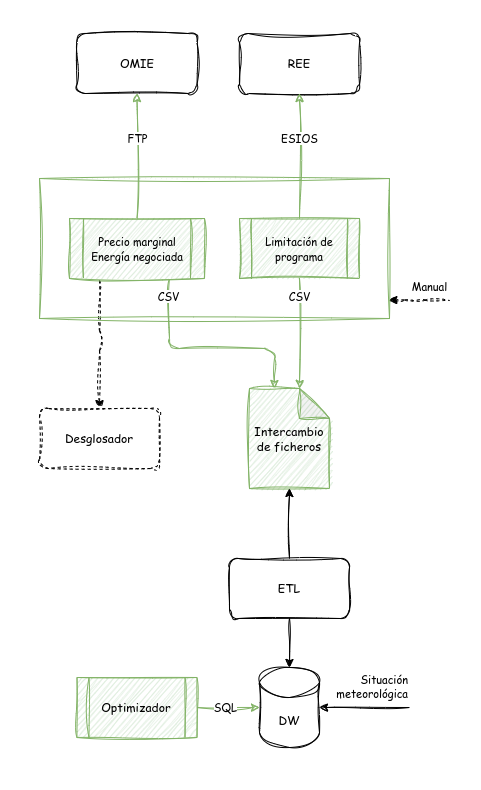
\includegraphics[width=0.5\linewidth]{figures/arquitectura-mercado.png}
  \caption{Arquitectura desacoplada del proceso de extracción, transformación y carga.}
  \label{fig:arquitectura-mercado}
\end{figure}

Esta arquitectura resulta ser un requisito para integrarse con herramientas internas ya existentes y, como ventaja adicional, proporciona una gran robustez frente a incidencias en las fuentes de datos.

Se han desarrollado dos programas principales en Python, uno para cada fuente de datos, que se ejecutan de forma periódica según los horarios de publicación de los ficheros de cada mercado según el cierre de los mismos para el que obtener los datos, si es aplicable.

La adquisición de datos de OMIE, aunque dispone de una interfaz web, no es apta para una integración automatizada. Por ello, la comunicación se realiza a través del servidor FTP que OMIE proporciona a los agentes de mercado registrados, ya que la API que la web pública usa no ofrece los datos en tiempo real debido a un periodo de confidencialidad.

El programa utiliza la librería Paramiko para establecer una conexión segura mediante SSH File Transfer Protocol con usuario y contraseña. Una vez conectado, el programa implementa una lógica para asegurar que siempre se obtiene la versión más reciente de cada fichero.

OMIE utiliza la nomenclatura \texttt{xxxxx\_aaaammdd[ss].v}, donde \texttt{xxxxx} es el nombre del fichero, \texttt{aaaa} es el año, \texttt{mm} es el mes, \texttt{dd} es el día y \texttt{ss} es la sesión del mercado, si es aplicable, y \texttt{v} es la versión del fichero.

Como se incluye una versión al final, el programa debe listar los ficheros para una fecha concreta, \textit{parsear} los nombres para identificar las versiones y descarga únicamente la más alta, ya que OMIE puede publicar correcciones o actualizaciones.

Para obtener las limitaciones de programa de Red Eléctrica, el enfoque es similar. Se debe utilizar la API privada de ESIOS (participa.esios), exclusiva para agentes de mercado, pues la API pública no proporciona la información en tiempo real. La comunicación se realiza mediante peticiones HTTP a través de la librería requests, utilizando autenticación de tipo Bearer con un token de acceso.

Una vez obtenidos los ficheros, que se presentan en formatos CSV específicos, la librería pandas se encarga de la transformación. El resultado es un fichero CSV cuyo formato se corresponde directamente con las filas a insertar en la base de datos de destino.

El formato de los datos de precios contiene las columnas fecha, hora y precio en euros por megavatio hora, pero es importante destacar que la columna hora representa el periodo de mercado porque anteriormente la granularidad de los mercados era exclusivamente horaria, según la tabla~\ref{tab:descripción-precio} y el contenido de la figura~\ref{fig:contenido-precio}.

\begin{table}[ht]
  \centering
  \begin{tabular}{|l|p{7.5cm}|l|}
    \hline
    Campo & Descripción & Valores válidos\\
    \hline
    Año & Año & I4 -- 20XX\\
    Mes & Mes & I2 -- 1 a 12\\
    Día & Día & I2 -- 1 a 31\\
    Hora & Hora & I2 -- 1 a 25\\
    MarginalPT & Precio marginal zona Portuguesa & F8.2 -- 0.0 a 99999.99\\
    MarginalES & Precio marginal zona Española & F8.2 -- 0.0 a 99999.99\\
    \hline
  \end{tabular}
  \caption{Descripción del formato de precios.}
  \label{tab:descripción-precio}
\end{table}

\begin{figure}
  \centering
  % 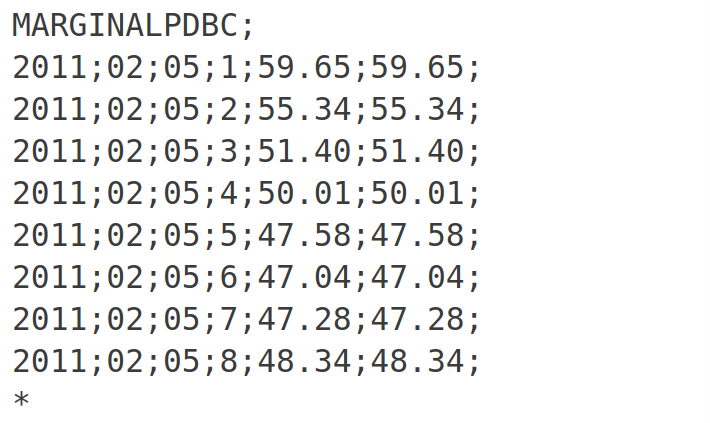
\includegraphics[width=0.5\linewidth]{figures/contenido-precio.png}
  \caption{Ejemplificación del contenido de los ficheros de precio.}
  \label{fig:contenido-precio}
\end{figure}

El desarrollo gestiona correctamente los husos horarios (horario local), ya que el mercado diario suele tener 24 periodos (granularidad horaria), pero puede tener 23 o 25 en días con cambio de hora. Análogamente, los mercados intradiarios, con granularidad cuartohoraria, tienen por lo general 96 periodos. Esto es debido a que el funcionamiento de los mercados siempre se realiza en horario local, sin excepción, por lo que no existen conflictos de solapamiento entre ellos.

El fichero de energía negociada contiene las columnas UP, fecha, hora y energía en megavatios hora. La presencia de la unidad programación es la razón fundamental del carácter confidencial de estos datos. Si un agente conociera los movimientos de las unidades que no controla, podría adaptar su estrategia en detrimento de la libre competencia, según la tabla~\ref{tab:descripción-energia} y el contenido de la figura~\ref{fig:contenido-energia}.

\begin{table}[ht]
  \centering
  \begin{tabular}{|l|p{5cm}|l|}
    \hline
    Campo & Descripción & Valores válidos\\
    \hline
    Año & Año & I4 -- 20XX\\
    Mes & Mes & I2 -- 1 a 12\\
    Día & Día & I2 -- 1 a 31\\
    Hora & Hora & I2 -- 1 a 25\\
    Código & Código de la unidad ofertante & A7\\
    Energía asignada & Energía asignada (MWh) & F7.1 – -99999.9 a 99999.9\\
    IdCBF & Identificador del Cont. Bilateral & I8 Vacío cuando es una oferta\\
    Tipo de oferta & Indicará que tipo de oferta es & I2 – 0 a 99\\
    NumOf & Indicará el número de oferta ó el de ejecución del contrato bilateral físico asociado a la unidad & I8 – -1 a 99999999\\
    \hline
  \end{tabular}
  \caption{Descripción del formato de energía negociada.}
  \label{tab:descripción-energia}
\end{table}

\begin{figure}
  \centering
  % 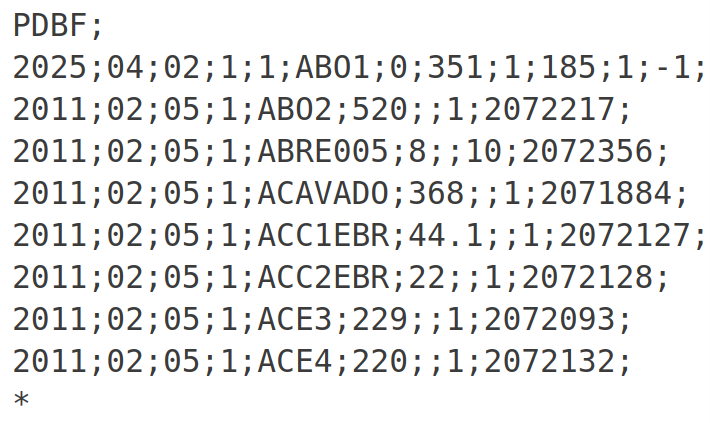
\includegraphics[width=0.5\linewidth]{figures/contenido-energia.png}
  \caption{Ejemplificación del contenido de los ficheros de energía.}
  \label{fig:contenido-energia}
\end{figure}

Aún con todo, existe un enorme problema que impide el uso de los resultados de la energía casada de forma directa. Esto se debe a que el sistema desarrollado necesita la información de la energía casada no por unidad de programación, sino por unidades físicas, de tal forma que se pueda arbitrar de forma independiente.

Para resolver este problema, se hace uso de una herramienta propietaria externa al desarrollo que es capaz de calcular los desgloses de la energía, convirtiendo la energía casada por unidad de programación a energía casada por unidad física. Para llevarlo a cabo debe hacer uso de información no disponible por el desarrollo, por lo la existencia de una herramienta del estilo es necesaria.

\begin{table}[ht]
  \centering
  \begin{tabular}{|l|p{5cm}|l|}
    \hline
    Campo & Descripción & Valores válidos\\
    \hline
    Año & Año & I4 -- 20XX\\
    Mes & Mes & I2 -- 1 a 12\\
    Día & Día & I2 -- 1 a 31\\
    Hora & Hora & I2 -- 1 a 25\\
    Código & Código de la unidad ofertante & A7\\
    Energía asignada & Energía asignada (MWh) & F7.1 – -99999.9 a 99999.9\\
    IdCBF & Identificador del Cont. Bilateral & I8 Vacío cuando es una oferta\\
    Tipo de oferta & Indicará que tipo de oferta es & I2 – 0 a 99\\
    NumOf & Indicará el número de oferta ó el de ejecución del contrato bilateral físico asociado a la unidad & I8 – -1 a 99999999\\
    \hline
  \end{tabular}
  \caption{Descripción del formato de las limitaciones técnicas.}
  \label{tab:descripción-limitaciones}
\end{table}

\begin{figure}
  \centering
  % 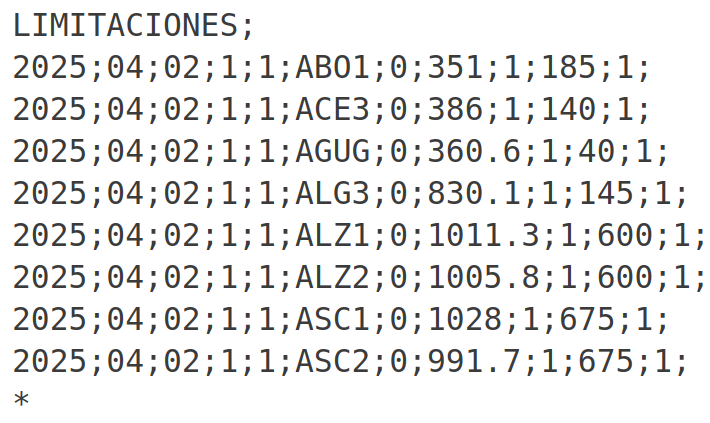
\includegraphics[width=0.5\linewidth]{figures/contenido-limitaciones.png}
  \caption{Limitaciones de programa a una instalación.}
  \label{fig:contenido-limitaciones}
\end{figure}

Junto a ello, el fichero de limitaciones de programa se estructura con las columnas fecha, hora, UP, UFI y valor. La lógica es que si el campo UFI tiene un valor, la limitación aplica exclusivamente a ese activo físico. Si está vacío, la limitación se aplica a la totalidad de la unidad de programación, como se puede ver en la table~\ref{tab:descripción-limitaciones} y en la figura~\ref{fig:contenido-limitaciones}

Una vez los datos residen en el data warehouse, el sistema de optimización los consume mediante consultas SQL. Sin embargo, la simple consulta no es suficiente, ya que las inserciones en la base de datos están sujetas a un versionado interno, independiente del versionado de los ficheros de origen.

Por esta razón, es necesario utilizar consultas analíticas de SQL que, específicamente, empleen funciones de ventana particionadas por la fecha y los periodos de mercado y las unidades de programación o físicas, si es aplicable, y las ordenen por la versión interna para garantizar que siempre se seleccione la versión más reciente de la información.

Además, se han realizado esfuerzos extensivos para reducir significativamente la latencia de estas consultas, un factor crítico para disminuir el tiempo de respuesta del sistema al completo.

El enfoque del sistema desarrollado consiste en construir consultas que filtran de manera agresiva sobre las columnas indexadas de las tablas base, asegurando que el motor de Oracle utilice planes de ejecución altamente eficientes.

Este método se adopta tras constatar que varias de las vistas de base de datos existentes, que teóricamente debían facilitar el acceso a la información, presentaban un rendimiento deficiente, que precisamente revelan que estas vistas utilizan constructos SQL subóptimos que impiden el uso correcto de los índices, resultando en tiempos de consulta inaceptables. Al interactuar directamente con las tablas subyacentes de forma optimizada, se logra una reducción drástica en los tiempos de respuesta.

Esta arquitectura desacoplada también facilita la gestión de incidencias. En ocasiones, OMIE o REE no publican los ficheros a tiempo. En estos casos, el proceso requiere una intervención manual en la que el agente de mercado contacta con la institución, que puede llegar a enviar el fichero por un canal alternativo como el correo electrónico.

Gracias al diseño, el operador puede procesar este fichero manualmente con los programas desarrollados y depositar el resultado en la ruta de intercambio, permitiendo que el flujo de datos se complete sin alterar el proceso de carga.
